\documentclass{report}
\usepackage[utf8]{inputenc}
\usepackage[top=1cm, bottom=2cm, left=2cm, right=2cm]{geometry}
\usepackage[francais]{babel}
\usepackage[T1]{fontenc}
\usepackage{graphicx}
\usepackage{subcaption}
\usepackage{listings}
\usepackage{hyperref}
\usepackage{wrapfig}

\title{Rapport}
\author{François PIAT}
\date{WEEK 9}

\begin{document}

\maketitle

\chapter*{Profiling}
\paragraph{Profilage des fonctions de MIRTK - Register}

- Soupçonnant des résultats non convergents, nous avons pris la décision d'arrêter les tests de profilage sur la fonction "register", du moins appliqué à des images 3D. Des images en 2 dimensions seront analysées par la suite, mais il était nécessaire de libérer le poste pour réaliser d'autres tests.\\

\paragraph{Analyse des performances de smooth-image TBB vs ArrayFire}

- Maintenant que smooth-image a pu être implémentée en remplaçant la dépendance de TBB par celle d'ArrayFire, il a fallu comparer les performances de chaque implémentation afin de vérifier la pertinence de l'inclusion d'ArrayFire au projet.\\
\\
L'implémentation intervenant principalement sur la fonction de convolution (cf rapport de la semaine précédente), voici ci-dessous les performances de convolution, en nombre total d'instructions : 
\begin{figure}[h!]
	\begin{center}
		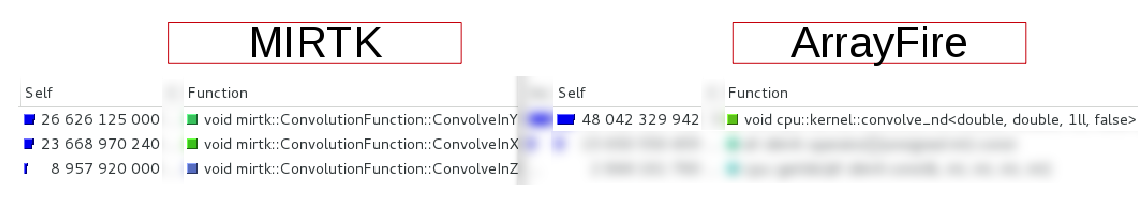
\includegraphics[width=19cm]{figures/MIRTK-AF-smoothimage.png}
	\end{center}	
	\caption{Performances de la convolution MIRTK vs ArrayFire}
	\label{Performances de la convolution MIRTK vs ArrayFire}
\end{figure}
\\Même si les performances ne sont pas grandement améliorées, on constate une simplification de la convolution, qui est faite par uniquement une fonction dans ArrayFire, et non une c\chapter*{Bazar}onvolution pour chaque dimension comme MIRTK le fait.

\chapter*{Implémentation}	

\paragraph{Stratégie}
-Pour permettre la transparence du code vis-à-vis de la machine qui l'éxecute, il a fallu ajouté au "main.cpp" des options en ligne de commande, permettant de choisir le back-end à utiliser pour éxecuter le code : CUDA (nvidia), OpenCL(autres GPU), ou CPU.\\

\paragraph{Problèmes}
- Conflit entre la bibliothèque "boost-program-options" pour l'ajout des options de back-end. On a donc implémenté dans un premier temps ces options de la même manière que les autres options de MIRTK.\\

\paragraph{Résultats}
- Utilisation des fonctions d'ArrayFire pour changer de back-end.\\
- La résolution des problèmes de compatibilité entre MIRTK et BOOST au niveau des options du programme s'est faite en incluant les options BOOST aux fonctions reconnues de MIRTK.\\

- En fin de semaine, on a basculé sur le canal TESTING de debian, ce qui a nécessité de refaire tous les builds déjà faits (MIRTK, Arrayfire...)\\



\end{document}